\documentclass[a4paper,12pt]{article}
\usepackage{graphicx}
\usepackage{amsmath}
\usepackage[margin=1in]{geometry}
\usepackage{amsmath, amssymb}
\usepackage{float}
\usepackage{caption}
\usepackage{subcaption}
\usepackage{xcolor}
\usepackage{fancyhdr}
\usepackage{array}
\usepackage{float}
\definecolor{darkskyblue}{rgb}{0.0, 0.5, 1.0}
\definecolor{skyblue}{RGB}{135, 206, 235}

\geometry{a4paper, top=0.7in, left=1in, right=1in, bottom=1in}

\begin{document}

\pagestyle{empty} % Start with empty page style

\thispagestyle{fancy} % Apply fancy style only to the first page
\fancyhf{} % Clear header and footer
\renewcommand{\headrulewidth}{0pt} % Remove header rule

\fancyhead[L]{% Left header
        
\includegraphics[width=8cm, height=1.7cm]{img3.png} 
        }
\fancyhead[R]{% Right header
    Name: K.Saisusmitha \\
    Batch: COMETFWC018 \\
    Date: 16 may 2025
}

\vspace{1cm}
\begin{center}

    {\LARGE \textbf{\textcolor{darkskyblue}{\\  GATE QUESTION \\ ECE 2009 Q38}}}
\end{center}

\vspace{-1cm} %adjust vertical space
\section*{\textcolor{blue}{\\Question}}
Q58)The following Karnaugh map represents a functionnF:
\vspace{1cm}
\noindent
\begin{center}
\textbf{The table represents a function \( F \):}
\end{center}
\vspace{1cm}
\noindent
\begin{center}
\begin{tabular}{|c|c|c|c|c|}
\hline
\( X \backslash YZ \) & 00 & 01 & 11 & 10 \\
\hline
0 & 1 & 1 & 1 & 0 \\
\hline
1 & 0 & 0 & 1 & 0 \\
\hline
\end{tabular}
\end{center}

\vspace{0.5em}
Which of the following circuits is a realization of the above function F?

\vspace{1em}
\begin{figure}[!h]
 \centering
     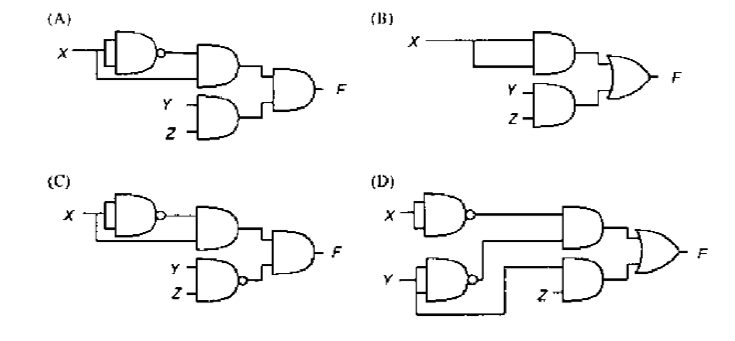
\includegraphics[width=8cm,height=6cm]{img2.png}
     \caption{}

 \end{figure}
 \section*{\textcolor{blue}{Solution}}
 
\textbf{Given K-map:}
\vspace{1cm}
\noindent
\begin{center}
\begin{tabular}{|c|c|c|c|c|}
\hline
\( X \backslash YZ \) & 00 & 01 & 11 & 10 \\
\hline
0 & 1 & 1 & 1 & 0 \\
\hline
1 & 0 & 0 & 1 & 0 \\
\hline
\end{tabular}
\end{center}
\vspace{0.5em}

From this K-map, the minterms where \( F = 1 \) are:

\begin{enumerate}
    \item \( m_0 \): \( X = 0, Y = 0, Z = 0 \Rightarrow \overline{X} \, \overline{Y} \, \overline{Z} \)
    \item \( m_1 \): \( X = 0, Y = 0, Z = 1 \Rightarrow \overline{X} \, \overline{Y} \, Z \)
    \item \( m_7 \): \( X = 1, Y = 1, Z = 1 \Rightarrow X Y Z \)
\end{enumerate}

So, the Boolean expression is:
\[
F = \overline{X} \, \overline{Y} \, \overline{Z} + \overline{X} \, \overline{Y} \, Z + X Y Z
\]

Group the first two terms:
\[
F = \overline{X} \, \overline{Y} (\overline{Z} + Z) + X Y Z = \overline{X} \, \overline{Y} + X Y Z
\]

So the correct simplified form is:
\[
\boxed{F = \overline{X} Y + Y Z}
\]

\textbf{Now examining the circuits in Q.53:}

\textbf{Circuit (A)} performs the following operations:
\begin{enumerate}
    \item First, invert \( X \) to get \( \overline{X} \)
    \item AND gate: \( \overline{X} \cdot Y = \overline{X} Y \)
    \item AND gate: \( Y \cdot Z = Y Z \)
    \item OR gate: \( \overline{X} Y + Y Z \)
\end{enumerate}
\textbf{This matches the simplified function.}

\section*{Final Answer:}
\[
\boxed{\text{Option (A)}}
\]

\end{document}
